\documentclass[12pt,reqno,final,pdftex]{amsart}\usepackage[]{graphicx}\usepackage[]{color}
%% maxwidth is the original width if it is less than linewidth
%% otherwise use linewidth (to make sure the graphics do not exceed the margin)
\makeatletter
\def\maxwidth{ %
  \ifdim\Gin@nat@width>\linewidth
    \linewidth
  \else
    \Gin@nat@width
  \fi
}
\makeatother

\definecolor{fgcolor}{rgb}{0.345, 0.345, 0.345}
\newcommand{\hlnum}[1]{\textcolor[rgb]{0.686,0.059,0.569}{#1}}%
\newcommand{\hlstr}[1]{\textcolor[rgb]{0.192,0.494,0.8}{#1}}%
\newcommand{\hlcom}[1]{\textcolor[rgb]{0.678,0.584,0.686}{\textit{#1}}}%
\newcommand{\hlopt}[1]{\textcolor[rgb]{0,0,0}{#1}}%
\newcommand{\hlstd}[1]{\textcolor[rgb]{0.345,0.345,0.345}{#1}}%
\newcommand{\hlkwa}[1]{\textcolor[rgb]{0.161,0.373,0.58}{\textbf{#1}}}%
\newcommand{\hlkwb}[1]{\textcolor[rgb]{0.69,0.353,0.396}{#1}}%
\newcommand{\hlkwc}[1]{\textcolor[rgb]{0.333,0.667,0.333}{#1}}%
\newcommand{\hlkwd}[1]{\textcolor[rgb]{0.737,0.353,0.396}{\textbf{#1}}}%
\let\hlipl\hlkwb

\usepackage{framed}
\makeatletter
\newenvironment{kframe}{%
 \def\at@end@of@kframe{}%
 \ifinner\ifhmode%
  \def\at@end@of@kframe{\end{minipage}}%
  \begin{minipage}{\columnwidth}%
 \fi\fi%
 \def\FrameCommand##1{\hskip\@totalleftmargin \hskip-\fboxsep
 \colorbox{shadecolor}{##1}\hskip-\fboxsep
     % There is no \\@totalrightmargin, so:
     \hskip-\linewidth \hskip-\@totalleftmargin \hskip\columnwidth}%
 \MakeFramed {\advance\hsize-\width
   \@totalleftmargin\z@ \linewidth\hsize
   \@setminipage}}%
 {\par\unskip\endMakeFramed%
 \at@end@of@kframe}
\makeatother

\definecolor{shadecolor}{rgb}{.97, .97, .97}
\definecolor{messagecolor}{rgb}{0, 0, 0}
\definecolor{warningcolor}{rgb}{1, 0, 1}
\definecolor{errorcolor}{rgb}{1, 0, 0}
\newenvironment{knitrout}{}{} % an empty environment to be redefined in TeX

\usepackage{alltt}
%% DO NOT DELETE OR CHANGE THE FOLLOWING TWO LINES!
%% $Revision$
%% $Date$
\usepackage[round,sort,elide]{natbib}
\usepackage{graphicx}
\usepackage{times}
\usepackage{rotating}
\usepackage{subfig}
\usepackage{color}
\newcommand{\aak}[1]{\textcolor{cyan}{#1}}
\newcommand{\mab}[1]{\textcolor{red}{#1}}
\newcommand{\cec}[1]{\textcolor{blue}{#1}}

\setlength{\textwidth}{6.25in}
\setlength{\textheight}{8.75in}
\setlength{\evensidemargin}{0in}
\setlength{\oddsidemargin}{0in}
\setlength{\topmargin}{-.35in}
\setlength{\parskip}{.1in}
\setlength{\parindent}{0.3in}

%% cleveref must be last loaded package
\usepackage[sort&compress]{cleveref}
\newcommand{\crefrangeconjunction}{--}
\crefname{figure}{Fig.}{Figs.}
\Crefname{figure}{Fig.}{Figs.}
\crefname{table}{Table}{Tables}
\Crefname{table}{Tab.}{Tables}
\crefname{equation}{Eq.}{Eqs.}
\Crefname{equation}{Eq.}{Eqs.}
\crefname{appendix}{Appendix}{Appendices}
\Crefname{appendix}{Appendix}{Appendices}
\creflabelformat{equation}{#2#1#3}

\theoremstyle{plain}
\newtheorem{thm}{Theorem}
\newtheorem{corol}[thm]{Corollary}
\newtheorem{prop}[thm]{Proposition}
\newtheorem{lemma}[thm]{Lemma}
\newtheorem{defn}[thm]{Definition}
\newtheorem{hyp}[thm]{Hypothesis}
\newtheorem{example}[thm]{Example}
\newtheorem{conj}[thm]{Conjecture}
\newtheorem{algorithm}[thm]{Algorithm}
\newtheorem{remark}{Remark}
\renewcommand\thethm{\arabic{thm}}
\renewcommand{\theremark}{}

\numberwithin{equation}{part}
\renewcommand\theequation{\arabic{equation}}
\renewcommand\thesection{\arabic{section}}
\renewcommand\thesubsection{\thesection.\arabic{subsection}}
\renewcommand\thefigure{\arabic{figure}}
\renewcommand\thetable{\arabic{table}}
\renewcommand\thefootnote{\arabic{footnote}}

\newcommand\scinot[2]{$#1 \times 10^{#2}$}
\newcommand{\code}[1]{\texttt{#1}}
\newcommand{\pkg}[1]{\textsf{#1}}
\newcommand{\dlta}[1]{{\Delta}{#1}}
\newcommand{\Prob}[1]{\mathbb{P}\left[#1\right]}
\newcommand{\Expect}[1]{\mathbb{E}\left[#1\right]}
\newcommand{\Var}[1]{\mathrm{Var}\left[#1\right]}
\newcommand{\dd}[1]{\mathrm{d}{#1}}
\newcommand{\citetpos}[1]{\citeauthor{#1}'s \citeyearpar{#1}}
\IfFileExists{upquote.sty}{\usepackage{upquote}}{}
\begin{document}



\section*{Changes from previous version}

Previously, the fitting algorithm had significant problems attempting to fit even simulated datasets.
I spent a lot of time trying to figure out why, and discovered a number of problems that I have fixed in the current version of both the model and the fitting algorithm.
Here's a brief list of the changes:
\begin{enumerate}
\item Previously, I assumed a Poisson distribution of measurement error. This is convenient because it is discrete and because it has no parameters to estimate (because the variance is equal to the mean). However, because we are measuring cumulative reproduction, this creates huge problems for fitting. For example, if the model-predicted cumulative reproduction was 50, and the observed cumulative reproduction was 45, I evaluated the likelihood using the call \texttt{dpois(x=45, lambda=50)}, so the measurement error variance was equal to 50! Basically, the Poisson has a variance that is far too high, given that observed reproduction is actually likely to have low measurement error - it's pretty easy to count babies! Now I am assuming normally distributed error.
\item In the previous version, there were issues with individuals shrinking. In particular, the DEB model tracks the dynamics of structural weight $W$ and reserves $E$. Structural weight is related to structural length $L$ as $L = W^{1/3}$. However, feeding is related to \emph{observed} length, $L_{obs}$. Thus I need to specify a relationship between the DEB variables and structural length. Often it is assumed that structural length is equal to observed length (e.g., $L=L_{obs}$). But length-weight regressions for \emph{Daphnia} do not suggest that this is true. For example, Nisbet et al. report that the scaling of observed length with observed weight has an exponent of 2.4, not 3. Since observed weight is the sum of structural mass and reserves, I assumed that $L_{obs} = ((W+E)/\xi)^{1/q}$, where $\xi$ and $q$ are regression parameters. However, this can make really weird things happen to weight between observations. For example, if you measure length on day 5 and day 10, then all that matters to the fitting is the value of $L_{obs}$ on day 5 and day 10 - between those dates, $L_{obs}$ can make biologically unreasonable excursions. For example, if there is a spike in $E$ between day 5 and 10 that quickly decays, $L_{obs}$ will also rapidly increase and decrease. So long as $E$ (and $L_{obs}$) have fallen by day 10, the fitting algorithm won't care about that spike. But biologically, it doesn't make any sense. This was especially problematic when I tried to estimate the initial value of both $W$ and $E$, because you could have high likelihood parameter sets where the initial $L_{obs}$ was 5mm (because $E$ was huge, and then rapidly decayed), and the animal just shrank from birth until the first measurement. Now I am assuming that $L_{obs} = (W/\xi)^{1/q}$ - the dynamics of $W$ are much less sensitive to the environment, which better matches with the insensitivity that we observe in $L_{obs}$. Moreover, $W$ doesn't fluctuate nearly as rapidly as does $E$.
\item Previously, I showed that it was essentially impossible to estimate the cost of reproduction $E_R$ while simultaneously estimating the allocation to growth $\kappa$ and the assimilation efficiency $\rho$ - the algorithm could arbitrarily slide these parameters around, making them essentially impossible to estimate simultaneously. However, I realized that there is actually some independent information about the cost of reproduction, which is that the cost of reproduction should be related to the initial values of reserves and structural mass. Now I am estimating the cost of reproduction, but assuming that $E_R = E(0) + W(0)$ to help constrain the fitting. I am using a standard DEB assumption to relate $E(0)$ and $W(0)$, which is that, at birth, $E(0)/W(0)$ is equal to the maximum reserve density, which is equal to $\rho/\nu$ (where $\rho$ is the assimilation efficiency and $\nu$ is the ``energy conductance'').
\end{enumerate}

Thus, the model that I am fitting is the following:
\begin{align}
\frac{dF}{dt} &= I_{max} \frac{F}{F_h+F} L_{obs}^g, \\
\frac{dE}{dt} &= \rho \epsilon V I_{max} \frac{F}{F_h+F} L_{obs}^g - P_C, \\
\frac{dW}{dt} &= \kappa P_C - k_m W, \\
\frac{dR}{dt} &= \frac{(1-\kappa) P_C}{E_R}, \text{ where} \\
P_C &= \frac{E (\nu/L + k_m)}{1 + \kappa E/W}, \\
L &= W^{1/3}, \\
L_{obs} &= (\frac{W}{\xi})^{1/q},
F(0) &= F_0, \\
E(0) &= \frac{\rho W(0)}{\nu}, \\
W(0) &= \frac{E_R}{1+\rho/\nu}, \\
R(0) &= 0.
\end{align}

The only aspects of this model that diverge from the standard DEB model (other than those discussed above) is the assumption that mobilization rate $P_C$ depends on structural length, whereas ingestion depends on observed length, and that there is no ``maturity maintenance.''

Of the parameters of this model, many are fixed:
\begin{align}
\epsilon &= 4.45 \times 10^{-8} \text{ carbon content of algae}, \\
V &= 30 \text{ volume of the experimental container}, \\
\xi &= 0.00262 \text{ length-weight regression coefficient (from Nisbet et al. 2004)}, \\
q &= 2.4 \text{ length-weight regression exponent (from Nisbet et al. 2004)}, \\
\nu &= 10 \text{ energy conductance}.
\end{align}

Other the $\nu$, the other parameters can be determined on the basis of other data.
My previous fitting attempts (as well as the results from other DEB fitting studies) suggest that the fitting results are basically insensitive to the value of $\nu$, so I fix this at 10.
Two other parameters are set by the results of the feeding model fitting.
The algorithm estimates the value of $F_h$ (the half-saturation constant), but once the value of $F_h$ is specified, both the maximum ingestion rate $I_{max}$ and the length-feeding rate exponent $g$ are set.
Thus the only parameters that are estimated are $F_h$, $\rho$ (the assimilation efficiency), $\kappa$ (the fractional allocation to growth), $k_m$ (the somatic maintenance rate), $E_R$ (the cost of reproduction), and the standard deviations of normal distributions describing the error in measurement of length and reproduction, $\sigma_L$ and $\sigma_R$.

For this exercise, I simulated 25 datasets, varying the values of $F_h$, $\rho$, $\kappa$, $k_m$, $\nu$, $E_R$, and $F(0)$.
I also let the amount of food added each timestep be variable, with a mean of $F(0)=33333$ and a standard deviation of 15000.
The variability in food addition is meant to reflect the reality that food addition is not perfect, even though we assume that it is in the model.
With the standard deviation being so high, this produces a lot of variation in food addition, with large impacts on growth and reproduction.
In reality, the standard deviation in food addition is probably much less than this, so the simulation may be overly pessimistic!

You can see in Fig. \ref{fig:rep-cost-est-2} that, overall, the algorithm does a pretty good job estimating all of the parameters.
The estimates are very close to the true values for almost every parameter and every dataset, as the the true value and estimate pairs are closely scattered around the one-to-one line.
In fact, there were only a few datasets where the algorithm really failed to estimate parameter reasonably well.

\begin{knitrout}\scriptsize
\definecolor{shadecolor}{rgb}{0.969, 0.969, 0.969}\color{fgcolor}\begin{figure}

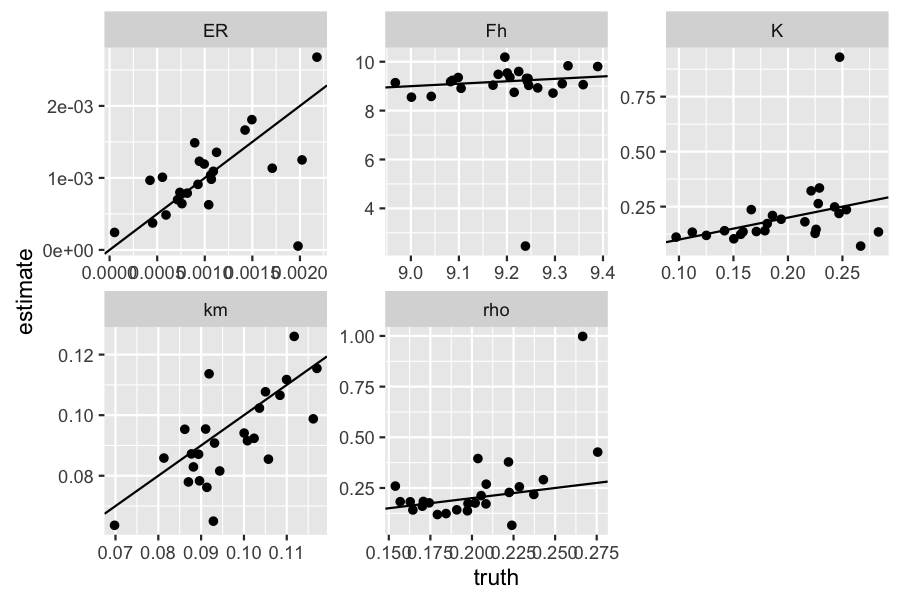
\includegraphics[width=\linewidth]{figure/rep-cost-est-2-1} \hfill{}

\caption[The highest likelihood parameter estimate from fitting each of 25 parameter sets using the model with normal measurement errors]{The highest likelihood parameter estimate from fitting each of 25 parameter sets using the model with normal measurement errors. Note that here I am also estimating the cost of reproduction. The true parameter value is given by the x-axis value and the estimate is given by the y-axis value. The line is the one-to-one line for reference.}\label{fig:rep-cost-est-2}
\end{figure}


\end{knitrout}

Fig. \ref{fig:rel-error-25-2} shows the relative (fractional) error for each parameter, organized by dataset.
For some of these datasets, we can understand what was going on that caused the parameter estimate to be so badly off.
For example, dataset 13 produced an estimate of assimilation efficiency that was much too high (the true value was 0.27 and the estimate was 0.99), an estimate of cost of reproduction that was too high (the true value was 5.2e-3 and the etimate was 2.4e-4), and an estimate of the observation error in reproduction that was much too high (the true value was 2 and the estimate was 134).

\begin{knitrout}\scriptsize
\definecolor{shadecolor}{rgb}{0.969, 0.969, 0.969}\color{fgcolor}\begin{figure}

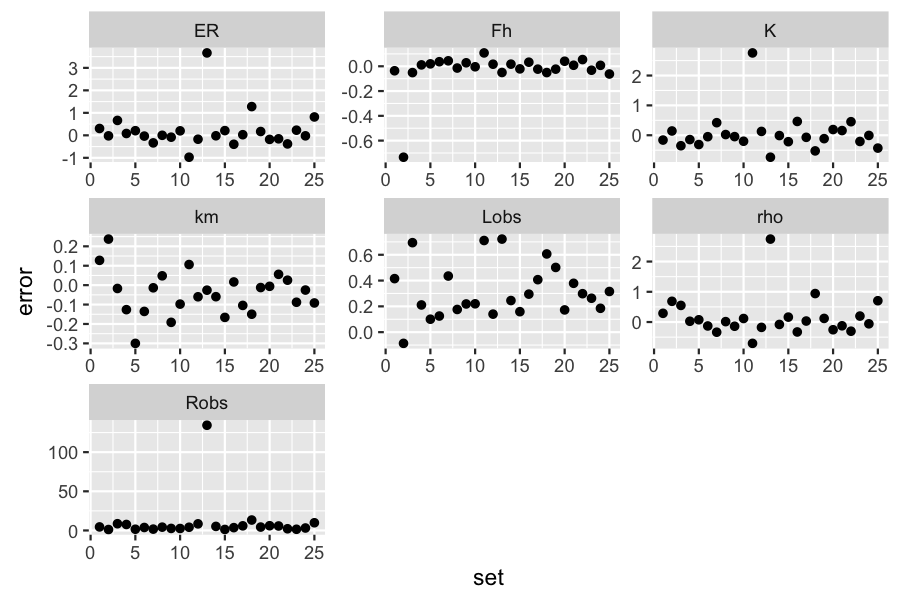
\includegraphics[width=\linewidth]{figure/rel-error-25-2-1} \hfill{}

\caption[Relative error in the parameter estimates for all 25 datasets]{Relative error in the parameter estimates for all 25 datasets.}\label{fig:rel-error-25-2}
\end{figure}


\end{knitrout}

\clearpage

However, if you look at the growth and reproduction trajectories for dataset 13 compared to all of the other growth and reproduction trajectories, you can see the problem.
Fig. \ref{fig:comparing-trajectories} shows that dataset 13 produced an animal that grew incredibly quickly and produced a \emph{huge} number of offspring.
This was because the true value of the cost of reproduction (which also sets the initial size of the offspring) was very low compared to all of the other parameter sets.
With such an extreme parameter value, the dataset itself was also extreme, and the algorithm struggled to find a good estimate.

\begin{knitrout}\scriptsize
\definecolor{shadecolor}{rgb}{0.969, 0.969, 0.969}\color{fgcolor}\begin{figure}

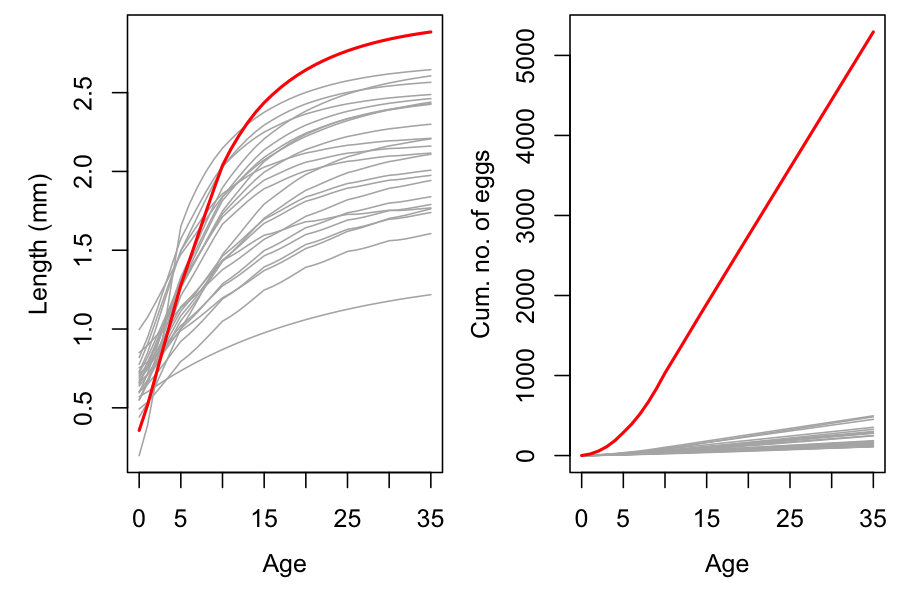
\includegraphics[width=\linewidth]{figure/comparing-trajectories-1} \hfill{}

\caption[The growth and reproduction trajectories at the true parameter values for dataset 13 (black) and all other datasets (grey)]{The growth and reproduction trajectories at the true parameter values for dataset 13 (black) and all other datasets (grey).}\label{fig:comparing-trajectories}
\end{figure}


\end{knitrout}

Another dataset that provided at least one very badly estimated parameter was dataset 2, where the half-saturation constant was estimated to be 11.7 when the true value was 10285.6.
Although it wasn't quite as large of an error, the estimate of assimilation efficiency was also quite off (the true value was 0.15 and the estimate was 0.26).
Looking at the growth and reproduction trajectories for dataset 2 compared to all of the other datasets (except 13, which we exclude to help with visualization, Fig. \ref{fig:comparing-trajectories-3}), you can see that this dataset was extreme in the other direction - the trajectory produced an animal that was tiny compared to every other animal in the dataset.

\begin{knitrout}\scriptsize
\definecolor{shadecolor}{rgb}{0.969, 0.969, 0.969}\color{fgcolor}\begin{figure}

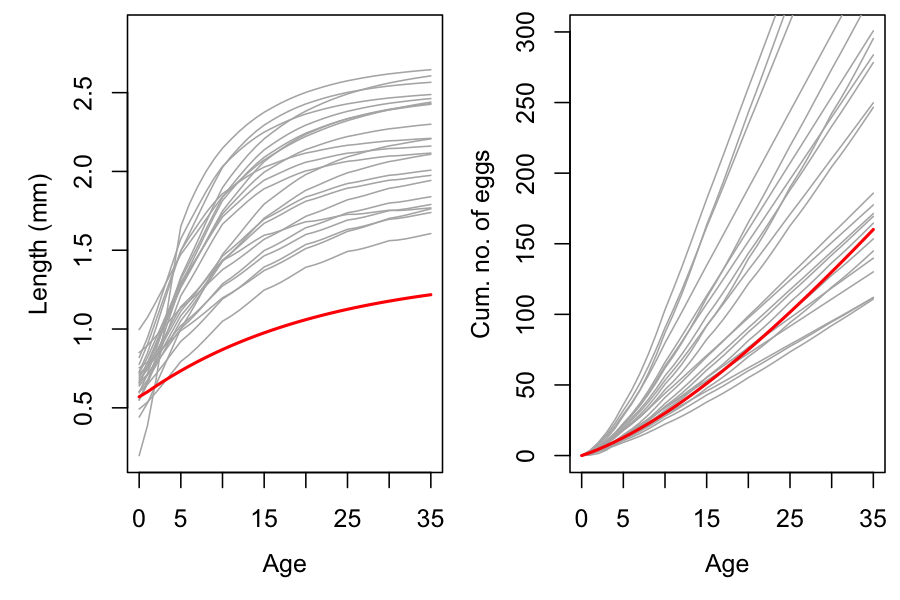
\includegraphics[width=\linewidth]{figure/comparing-trajectories-2-1} \hfill{}

\caption[The growth and reproduction trajectories at the true parameter values for dataset 2 (red) and all other parameter sets (grey)]{The growth and reproduction trajectories at the true parameter values for dataset 2 (red) and all other parameter sets (grey).}\label{fig:comparing-trajectories-2}
\end{figure}


\end{knitrout}

The final dataset that produced some bad parameter estimates was dataset 11, which produced an estimate of growth allocation $\kappa$ that was too high (the true value was 0.25 and the estimate was 0.93), you can see that again, the dataset was extreme, with the animal growing very rapidly to very large size and having very few offspring (Fig. \ref{fig:comparing-trajectories-2}).

\begin{knitrout}\scriptsize
\definecolor{shadecolor}{rgb}{0.969, 0.969, 0.969}\color{fgcolor}\begin{figure}

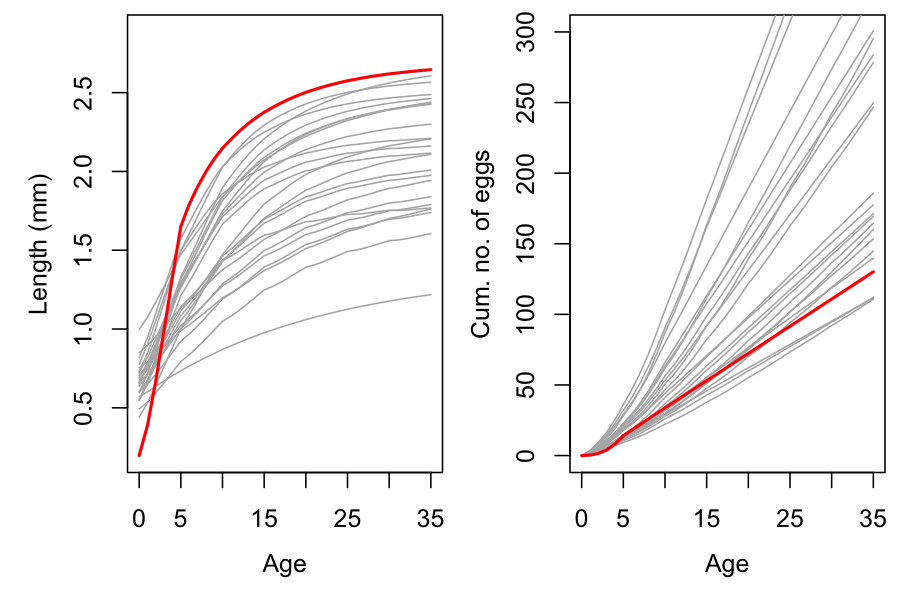
\includegraphics[width=\linewidth]{figure/comparing-trajectories-3-1} \hfill{}

\caption[The growth and reproduction trajectories at the true parameter values for dataset 11 (red) and all other datasets (grey)]{The growth and reproduction trajectories at the true parameter values for dataset 11 (red) and all other datasets (grey).}\label{fig:comparing-trajectories-3}
\end{figure}


\end{knitrout}

So, basically, the algorithm struggles to fit extreme datasets.
Interestingly, while this datasets are extreme, relative to the other datasets being fit, it is unclear why they should be hard to fit.
An examination of the true parameter values for each dataset can be somewhat illustrative (Fig. \ref{fig:comparing-parameters}).
In particular, as noted above, for the case of dataset 13, one of the parameter values was actually fairly extreme (cost of reproduction was very low).
For dataset 2, on the other hand, both the growth allocation $\kappa$ and the assimilation efficiency $\rho$ were very low.
Dataset 11, on the other hand, doesn't appear to be very unusual in terms of its parameter values.

\begin{knitrout}\scriptsize
\definecolor{shadecolor}{rgb}{0.969, 0.969, 0.969}\color{fgcolor}\begin{figure}

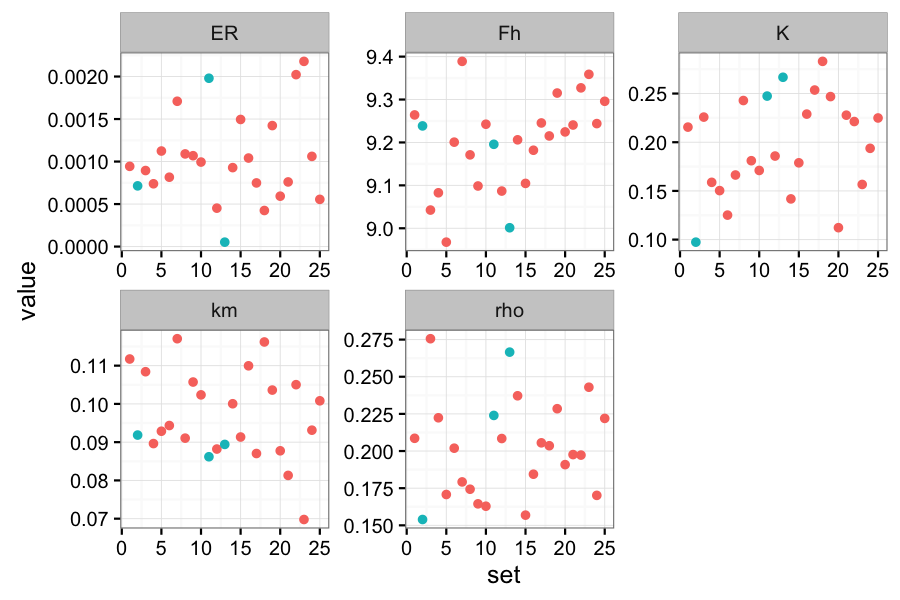
\includegraphics[width=\linewidth]{figure/comparing-parameters-1} \hfill{}

\caption[True parameter values for all 25 parameter sets]{True parameter values for all 25 parameter sets. The hard-to-fit parameter sets are colored blue.}\label{fig:comparing-parameters}
\end{figure}


\end{knitrout}

\clearpage

Regardless, if you remove these three extreme datasets, the plots of the estimates compared to the truth look great (Fig. \ref{fig:best-estimates}).
\begin{knitrout}\scriptsize
\definecolor{shadecolor}{rgb}{0.969, 0.969, 0.969}\color{fgcolor}\begin{figure}

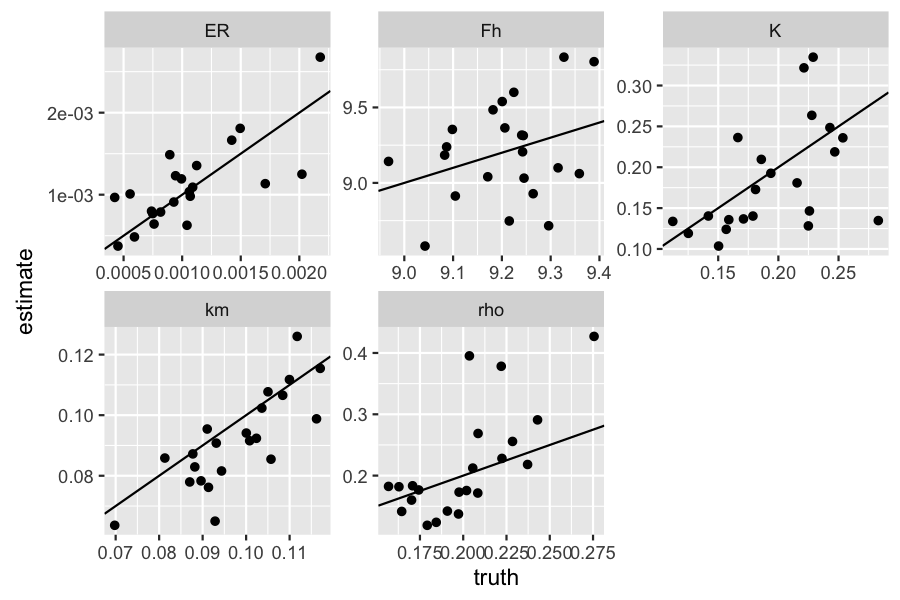
\includegraphics[width=\linewidth]{figure/best-estimates-1} \hfill{}

\caption[Looking at the estimates when you exclude the 3 datasets that were hard to fit]{Looking at the estimates when you exclude the 3 datasets that were hard to fit.}\label{fig:best-estimates}
\end{figure}


\end{knitrout}

\clearpage

I am wondering, however, whether I couldn't do better if I increased the size of the initial box of guesses and the number of estimates that I refine through Nelder-Mead.
In particular, I am wondering whether some parameter sets that are somewhat close to the true parameter set have lower likelihoods than other places in parameter space, and are thus excluded from the Nelder-Mead optimization, even though if they were optimized they would end up with higher likelihoods.
Another possibility, of course, is that the true parameter values are actually somewhat less likely than other places and, moreover, sit on a very steep, isolated peak in likelihood space, so that they are hard to find and hard to stay near.
I am going to explore this by initializing optimizations at the true parameter values and then seeing how the results of those optimizations compare with the results from the blind optimization.

Fig. \ref{fig:free-vs-truth-start} shows that, when you start the optimization algorithm at the true parameter values, the ML parameter estimates are closer to the truth (in almost every case) than those started blindly.

\begin{knitrout}\scriptsize
\definecolor{shadecolor}{rgb}{0.969, 0.969, 0.969}\color{fgcolor}\begin{figure}

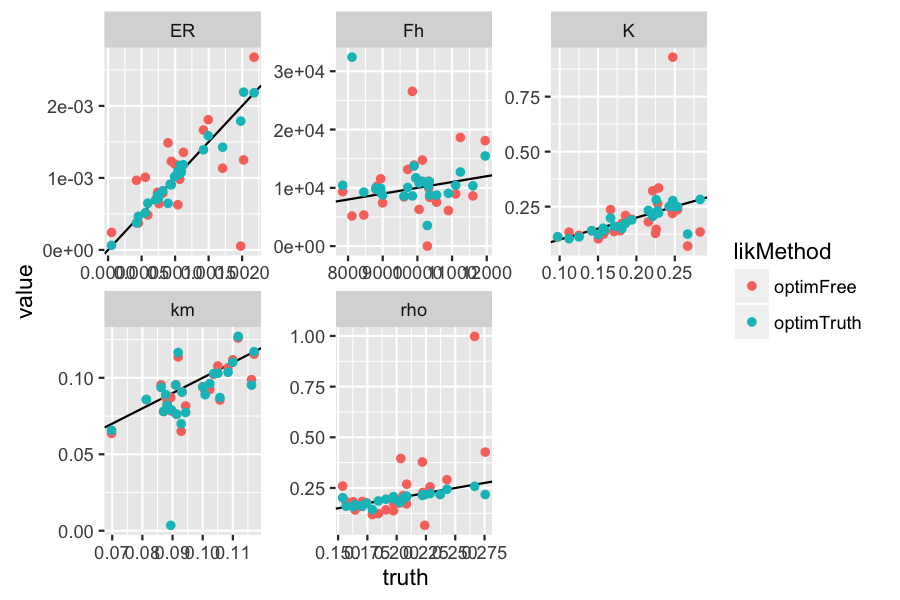
\includegraphics[width=\linewidth]{figure/free-vs-truth-start-1} \hfill{}

\caption[Comparing the true parameter values (x-axis) against the parameter estimates when the optimization algorithm starts from naive guesses and when the algorithm starts at the true parameter values]{Comparing the true parameter values (x-axis) against the parameter estimates when the optimization algorithm starts from naive guesses and when the algorithm starts at the true parameter values.}\label{fig:free-vs-truth-start}
\end{figure}


\end{knitrout}

More interesting, however, are the results of the likelihood calculation.
The likelihoods of the parameter estimates found either by the full optimization process or by starting at the true parameter values are so close that they lie on top of one another for almost every dataset (Fig. \ref{fig:lik-comparison}).
However, the likelihoods of the true parameter sets themselves are often much, much smaller.
This is most evident for parameter set 13, but you can see huge log-likelihood differences across the board.
However, it is also important to note that, in all but one case, the likelihood found by the full optimization is at least as good as the likelihood found by starting at the true parameter values (Fig. \ref{fig:lik-comparison-2}), although the differences are almost always very tiny.

\begin{knitrout}\scriptsize
\definecolor{shadecolor}{rgb}{0.969, 0.969, 0.969}\color{fgcolor}\begin{figure}

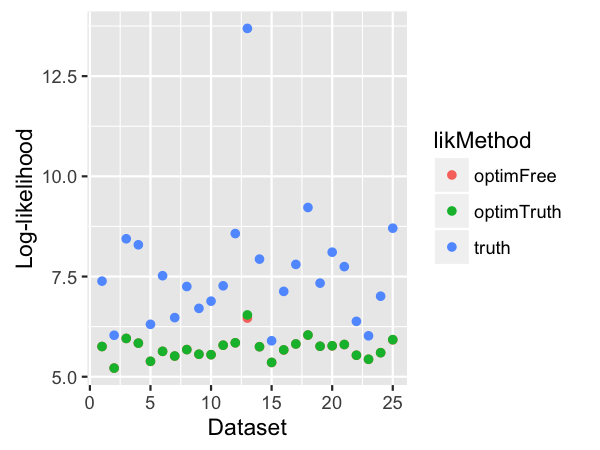
\includegraphics[width=\linewidth]{figure/lik-comparison-1} \hfill{}

\caption[Comparing the likelihood of the true parameter values to the likelihoods obtained by the fitting algorithm when initialized completely randomly and when initialized at the true parameter values]{Comparing the likelihood of the true parameter values to the likelihoods obtained by the fitting algorithm when initialized completely randomly and when initialized at the true parameter values.}\label{fig:lik-comparison}
\end{figure}


\end{knitrout}

\begin{knitrout}\scriptsize
\definecolor{shadecolor}{rgb}{0.969, 0.969, 0.969}\color{fgcolor}\begin{figure}

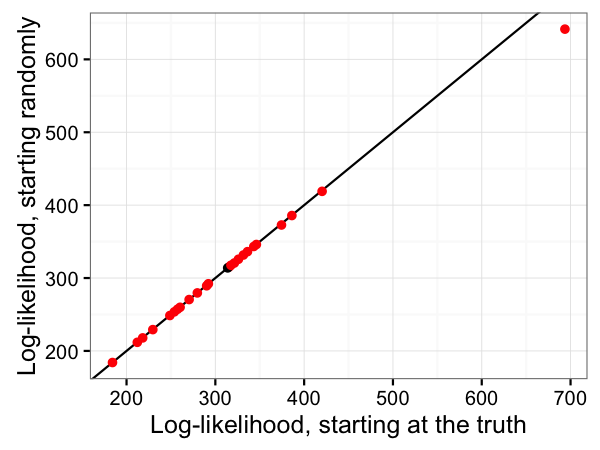
\includegraphics[width=\linewidth]{figure/lik-comparison-2-1} \hfill{}

\caption[Comparing the log-likelihoods found via the optimization algorithm starting without any constraint versus that found from starting at the true parameter values]{Comparing the log-likelihoods found via the optimization algorithm starting without any constraint versus that found from starting at the true parameter values. Red points indicate datasets where the likelihood was lower for the free start.}\label{fig:lik-comparison-2}
\end{figure}


\end{knitrout}

\clearpage

Thus it appears to be generally true that there will be multiple parameter sets that give rise to nearly identical likelihoods, making it impossible to know, in general, which is closer to the truth.
However, the overall message from this fitting is pretty encouraging, as most of the parameter estimates are close to the truth and the algorithm is finding high likelihood parameter sets.
The problem of ridges in likelihood space is almost certain to be unavoidable.

Moreover, if I reduce the variability in the food addition (from a standard deviation of 15000 to just 5000, which is probably more realistic), the estimates improve further.
Fig. \ref{fig:rep-cost-est-3} shows the relative error in the parameter estimates for 25 parameter sets (note that all parameters are equal to the parameter sets above except for the variability in food addition).
As you can see, there is only one dataset with absolute relative error greater than one (dataset 13, which hugely overestimated the cost of reproduction and the observation error).
However, this is the parameter set that produced an individual that reproduced far more than any other, so this result is expected.
Otherwise, the parameter estimates look good for basically every parameter.

\begin{knitrout}\scriptsize
\definecolor{shadecolor}{rgb}{0.969, 0.969, 0.969}\color{fgcolor}\begin{figure}

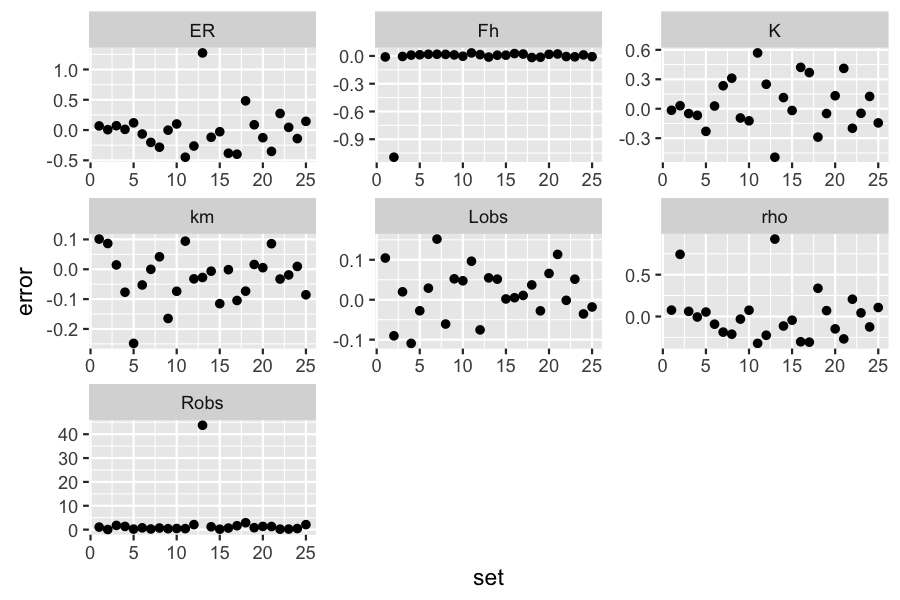
\includegraphics[width=\linewidth]{figure/rep-cost-est-3-1} \hfill{}

\caption[Relative error in parameter estimates for 25 parameter sets when the variability in food addition is reduced]{Relative error in parameter estimates for 25 parameter sets when the variability in food addition is reduced.}\label{fig:rep-cost-est-3}
\end{figure}


\end{knitrout}

\end{document}
